\chapter{High Level Design}
Design is significant phase in development of software. It is basically a creative procedure which includes the description of the system organization, establishes that it satisfies the functional and non-functional system requirements. Larger systems divided down into smaller sub-systems contain services that are related to each other. The output in design phase describes the architecture of software to be used for the development of the common endpoint service. This section depicts the issues that are required to be covered or resolved before attempting to devise a complete design solution. The detailed design includes an explanation for all the modules. It throws light on the purpose, functionality, input and output. The software specification requirements have been studied to design an appropriate and efficient software to handle a multitude of users belonging to different user groups simultaneously accessing the system.

\section{Design Considerations}
There are several design consideration issues that need to be fixed before designing a solution for the system to be implemented. The following sections describe constraints that have heavy impact on the software, a method or approach used for the development and the architectural strategies. It also describes the overview of the system design.

    \subsection{General Constraints}
    General constraints which need to be considered are:

    \begin{itemize}
    \item The user should have access/authorization to use the system
    \item The user should have knowledge of the required inputs and the formats of the inputs
    \item The system must be tuned for the use-case before using it

    \end{itemize}

    \subsection{Development Methods}
    The design method employed is highlighted in this chapter. The data flow model has been the design method employed for development of the system. A data flow model is modeling system based on data transformation that takes place as the data is being processed. The notations used represent functional processing and data stores. Data flow models gives the better understanding of how data is associated with the particular process by tracking and providing the documentation.

    We have split up the project into independent modules which can be independently developed, tested and validated.


\section{Architectural Strategies}
The overall organization of the system and its high level structure is provided by this section and this section also provides the key insight into the mechanism and strategies used in system architecture. The overall architecture was designed keeping in mind the need for rapid-prototyping required for a project of this scale which needs to be accomplished in a fairly short period of time.

    \subsection{Programming Language}
    The system involves two major segments, the frontend and backend which are built using Python, Javascript, HTML, CSS. Python is a object oriented programming languages which support wide range of data types and application programming interface for handling the data. The user interfaces are developed using HTML, CSS and JavaScript.

    Other important packages which were vital for developing this project were OpenCV implementations of several image processing algorithms, Jupyter’s interactive python interpreter and NumPy package used for performing fast and vectorized operations on images.

    \subsection{User Interface Paradigm}
    The GUI of the system is a form based interface. It is light-weight and fairly simple to develop. However, it is built to only take valid input queries from the user. Therefore the UI paradigms which we wish to achieve are consistency, clarity and simplicity.

    \subsection{Error Detection and Recovery}
    Error detection and recovery is an important aspect of the implemented project. We have implemented user form validation in the very beginning of the pipeline. Almost all kinds of errors will be weeded out in the very beginning of the pipeline. Internal error detection is done using the exception handling clauses provided by Python and using plenty of datatype asserts wherever possible. Since the project is divided into clearly defined modules with pre-defined interfaces, debugging and detecting errors is very easy.

\section{System Architecture}
This section is focused on basic structure of model in the system. It aims to identify major modules in system and communication flow amongst these modules. The approach used for the development of the common endpoint service is object oriented wherein the system is classified into different objects, which represent real world entities. The architecture is depicted in the figure below.

\begin{figure}[H]
    \centering
    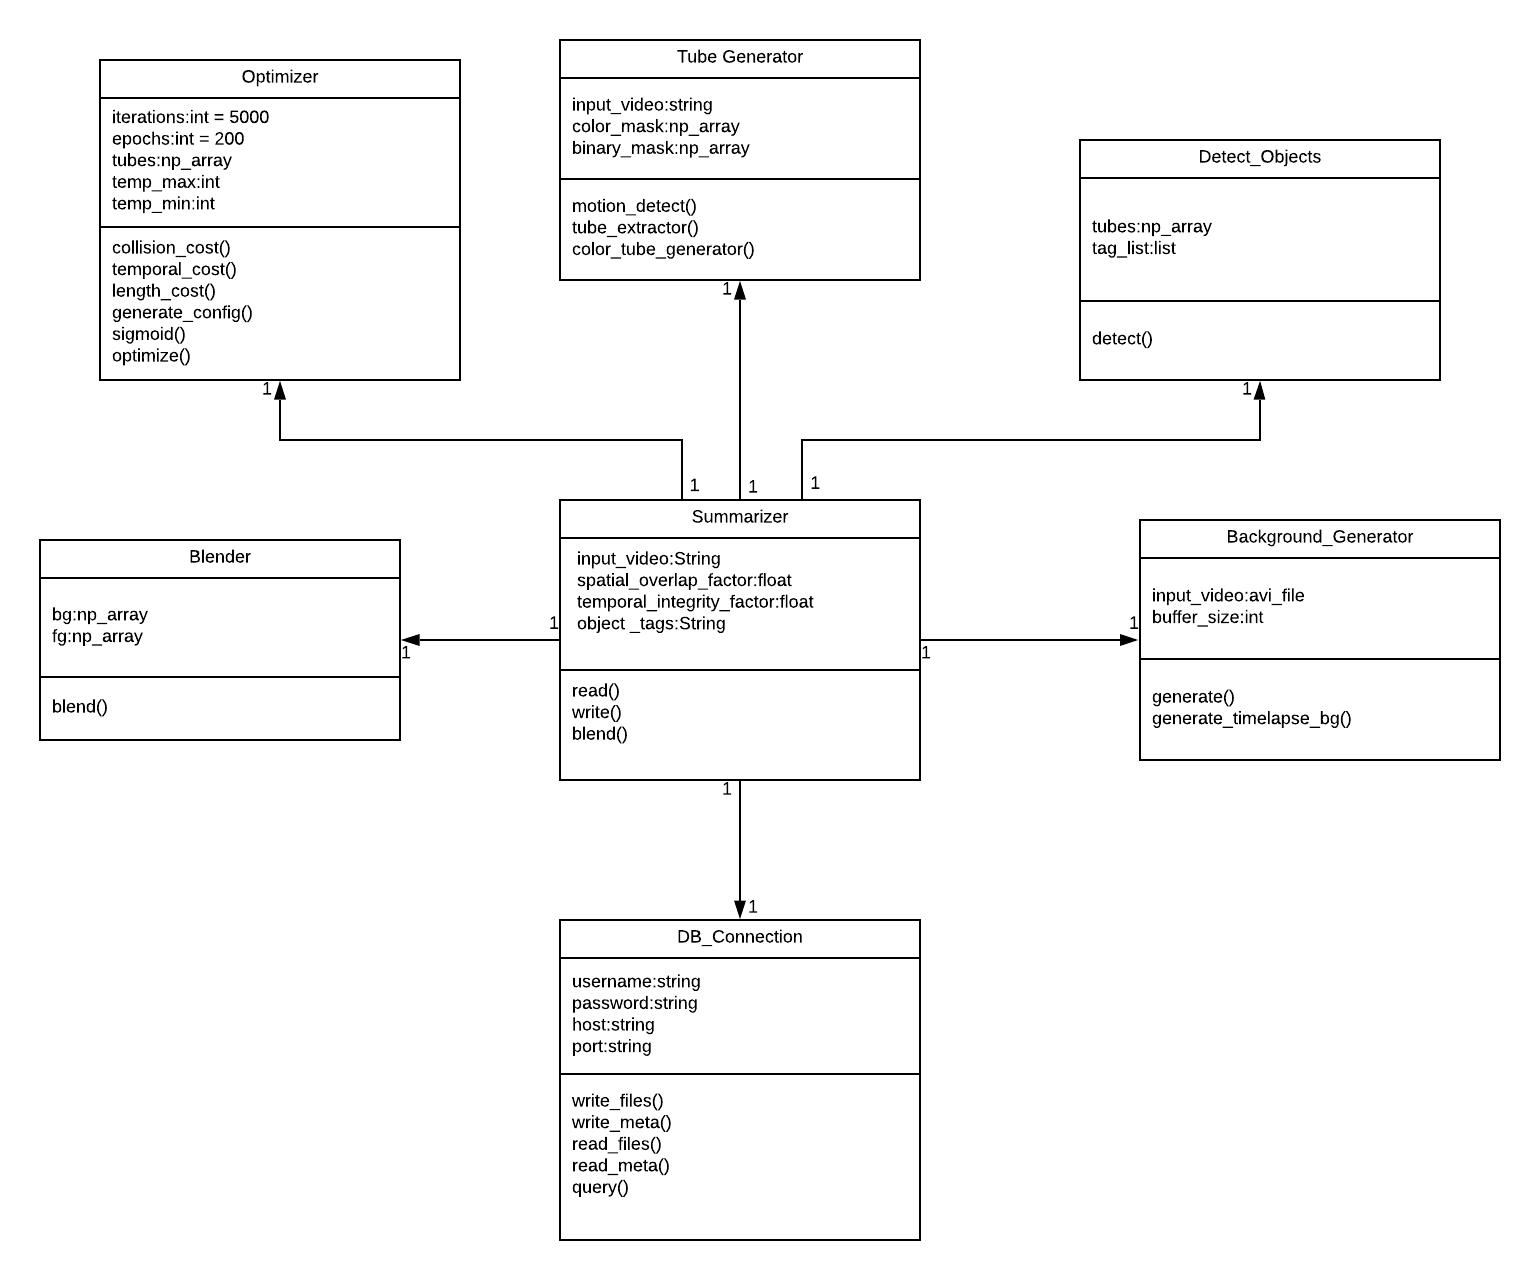
\includegraphics[scale=0.37]{uml.png}
    \caption{UML Class Diagram}
    \label{img:uml}
\end{figure}

The system architecture is as shown in Figure \ref{img:uml}. The central summarizer object creates objects other modules mentioned in the figure and uses them in a sequence mentioned in chapter 2. Each constructor of the classes defined above, have strict assert statements to ensure the data they receive are of the proper type before any kind of operations are performed on them.

\section{Data Flow Diagram}

A Data Flow Diagram (DFD) is graphical representation of the "flow" of data through an information system. Data Flow models describe how data flows through a sequence of processing steps. DFD is composed of four elements, which are process, data flow, external entity and data store. With data flow diagram, the users can easily to visualize the operations within the system, what can be accomplished using the system and implementation of the system. DFDs provide the end users an abstract idea regarding the data that is given as input to the system, the effect that the input will ultimately have upon the whole system.

The level 0 diagram shows the main data streams in the system. The level 1 diagram shows the input and output data in the two main processing pipelines. The level 2 diagram explains the data transformation in each pipeline step-by-step.

    \subsection{Data Flow Diagram – Level 0}

    The level 0 DFD describes general operation of the system. It represents the system and user and the inputs and outputs between the user and the system.

    \begin{figure}[H]
        \centering
        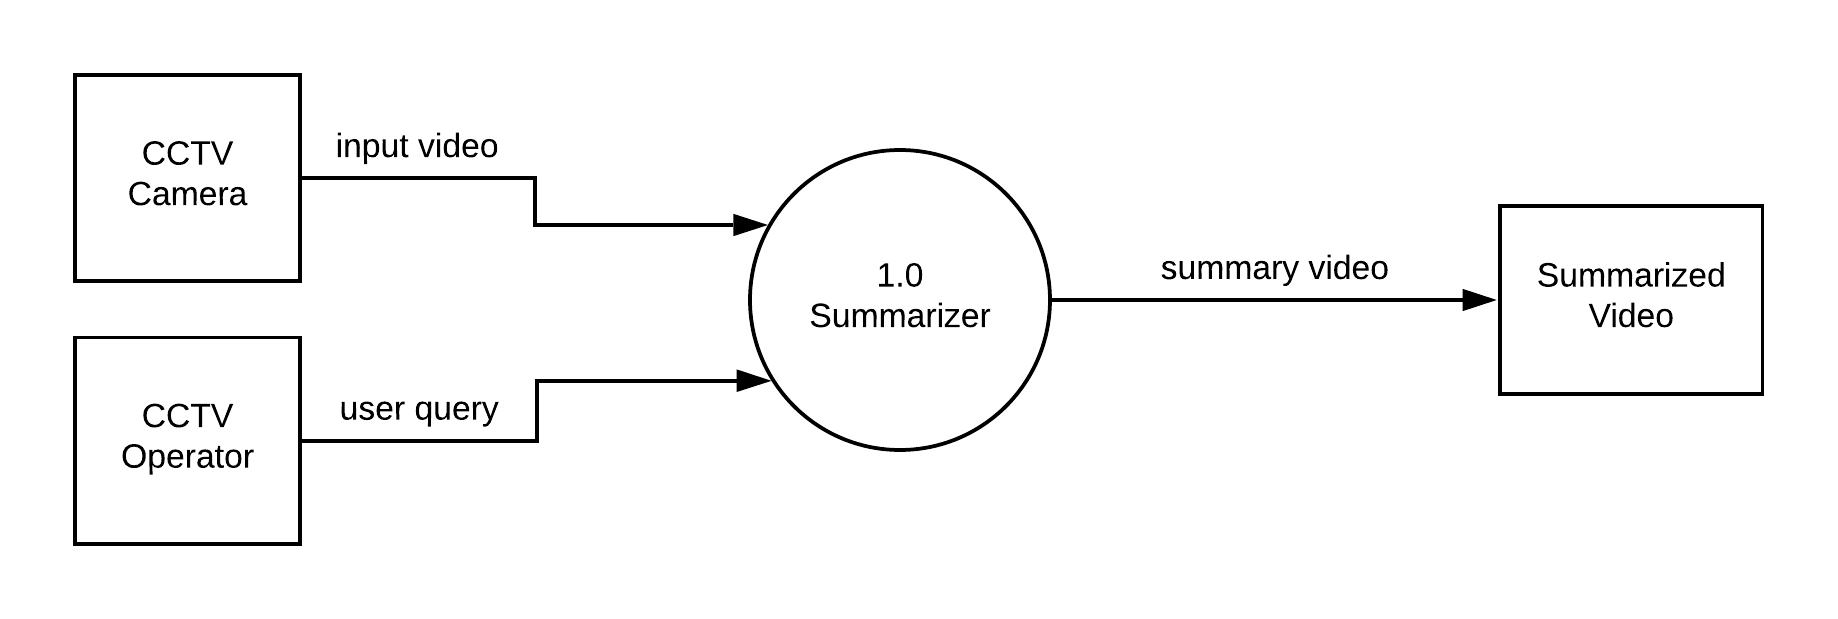
\includegraphics[scale=0.3]{dfd-lvl-0.png}
        \caption{Data Flow Diagram - Level 0 }
        \label{img:dfd-lvl-0}
    \end{figure}

    Figure \ref{img:dfd-lvl-0} gives an abstract representation of the system. The input video from CCTV is fed into the Summarizer which gives the video summary as output, based on the query from the CCTV operator/user.


    \subsection{Data Flow Diagram – Level 1}

    The Level 1 DFD describes the system more in detail than the Level 0 DFD. It specifies the two main phases involved in the system. This is as shown in fig \ref{img:dfd-lvl-1}.

    \begin{figure}[H]
        \centering
        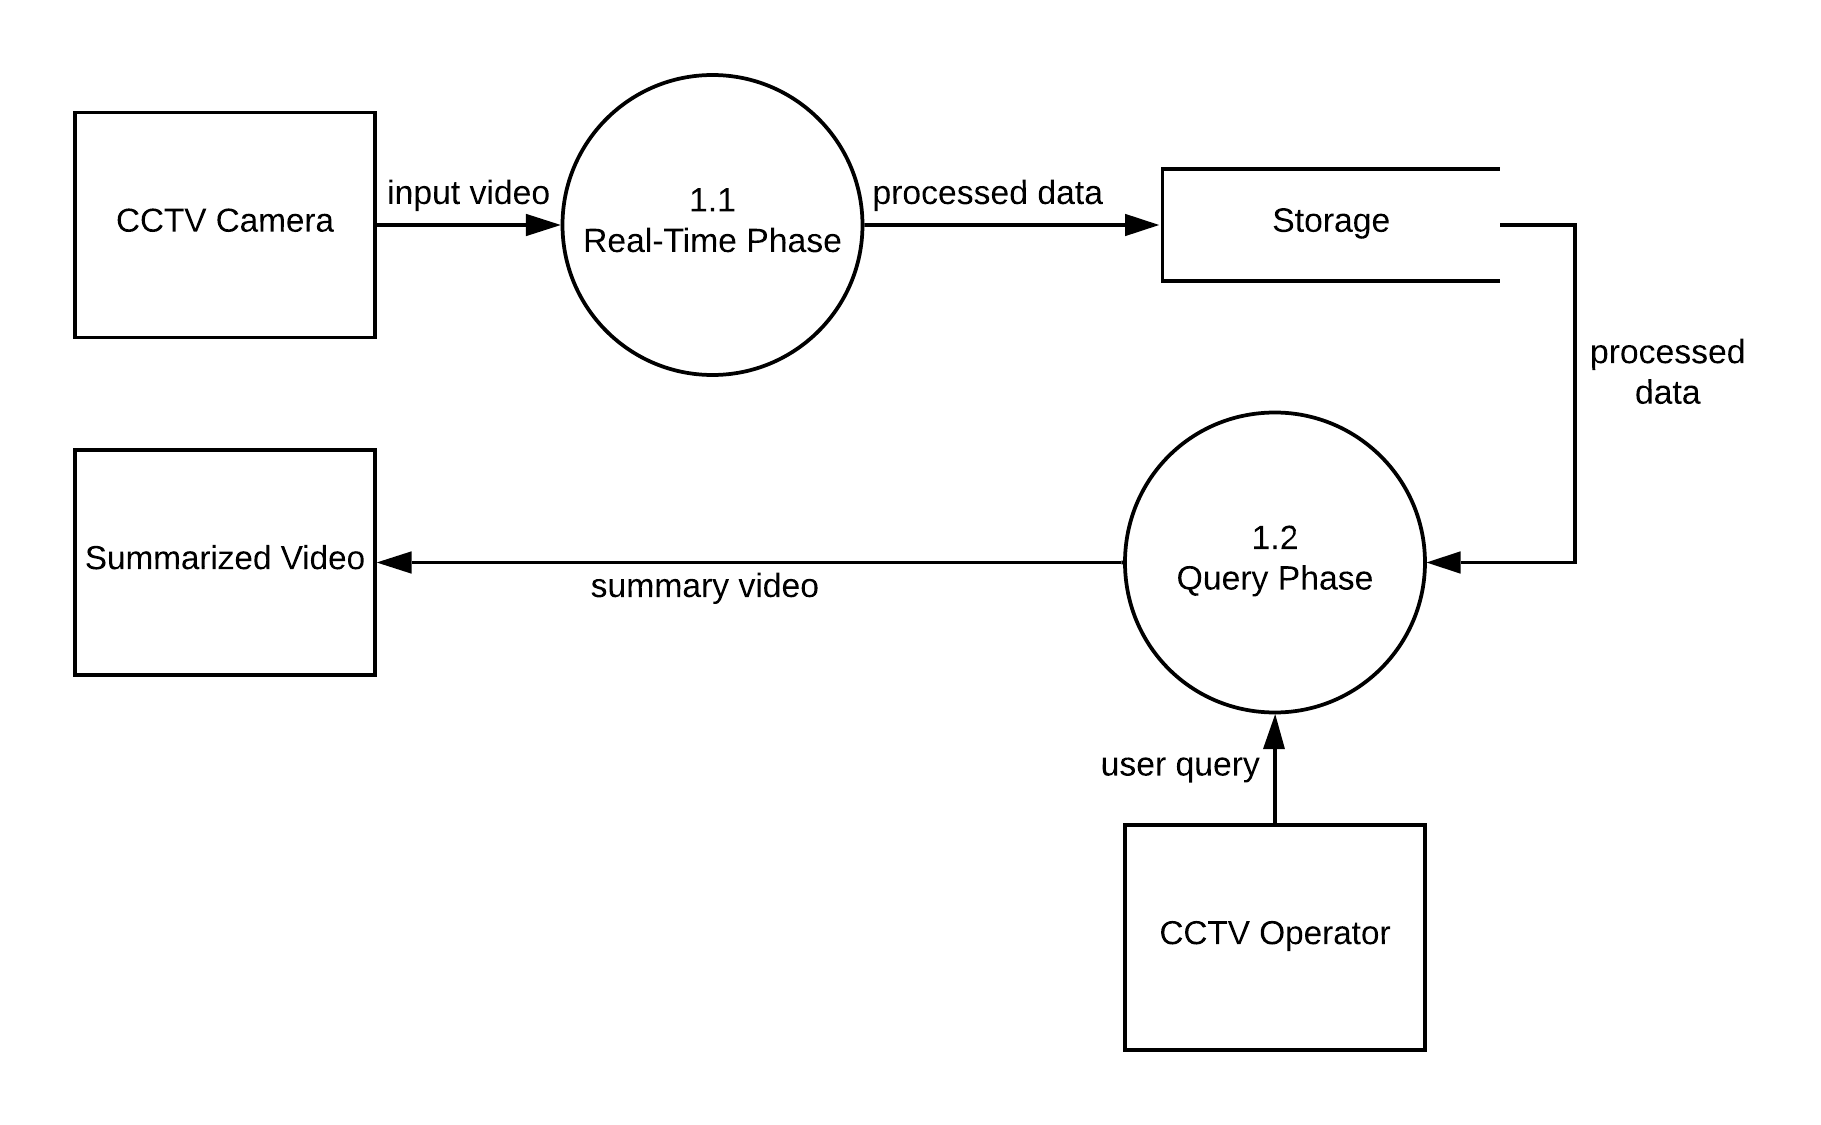
\includegraphics[scale=0.32]{dfd-lvl-1.png}
        \caption{Data Flow Diagram - Level 1 }
        \label{img:dfd-lvl-1}
    \end{figure}

    The real-time phase takes in the input video from the CCTV camera and processes the data for the next phase. Different methods like motion detection, background masking, tube extraction and object detection are applied on the given input video. The pre-processed data is then stored in the database. Next, a query is given as input for the next phase. Using the preprocessed data from phase one, a summarized video is generated.

    \subsection{Data Flow Diagram – Level 2}

    Figures \ref{img:dfd-lvl-21}, \ref{img:dfd-lvl-22} represent the level 2 data flow diagrams.

    The processes in level 1 are expanded here. The Level 2 DFD for Real-time phase of the video summarizer is shown in figure \ref{img:dfd-lvl-21}.

    \begin{figure}[H]
        \centering
        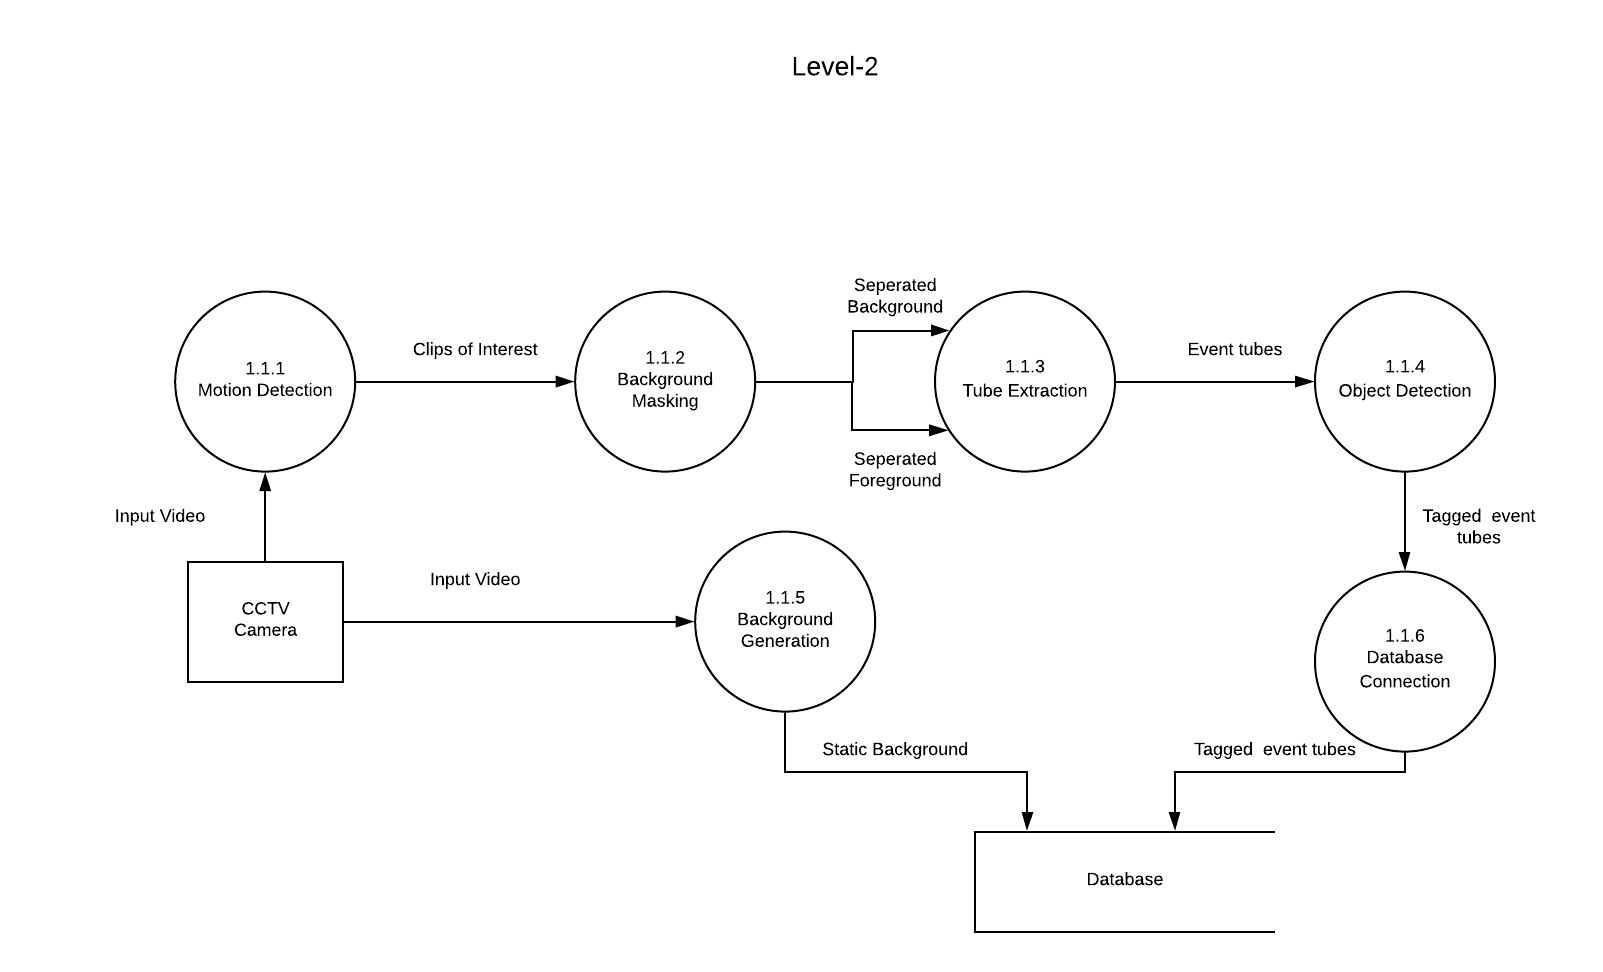
\includegraphics[scale=0.35]{dfd-lvl-21.png}
        \caption {Data Flow Diagram - Level 2 (Depth image processing)}
        \label{img:dfd-lvl-21}
    \end{figure}

    Motion is first detected frame by frame be using a threshold of number of active pixels in the binary mask. From these clips of interest, the foreground is extracted using MOG2. Events of interest are then extracted as tubes. YOLO object detector is then applied to these tubes to create tagged even tubes which are stored in the database. Simultaneously, a static background is generated from the input footage, which is also stored.

    \begin{figure}[H]
        \centering
        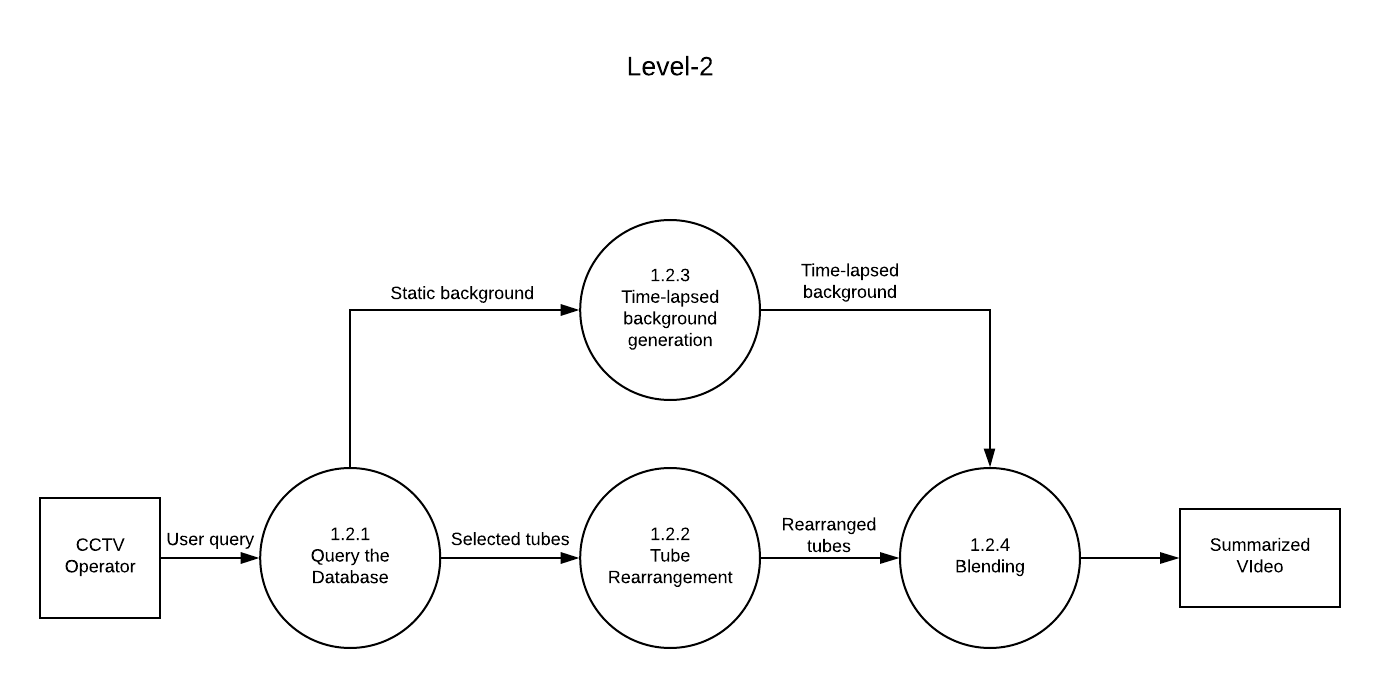
\includegraphics[scale=0.4]{dfd-lvl-22.png}
        \caption {Data Flow Diagram - Level 2 (Colour image processing)}
        \label{img:dfd-lvl-22}
    \end{figure}

    Figure \ref{img:dfd-lvl-22} shows level 2 DFD for Query phase of the Video Summarizer. Based on the user query, tubes of interest are first selected from the database. These tubes are then rearranged using Simulated Annealing.. While this process is being completed, a time-lapsed background is also formed. In the next step, the rearranged tubes are blended into the time-lapsed background by Poisson blending. The generated summarized video is then stored.

\section{Summary}
The above data models depict how data is processed by the system. This constitutes the analysis level. The notations applied above represent functional processing, data stores and data movement amongst the functions. The purpose of chapter is to describe major high- level processes (the two phases – Real time and Query) and their interrelation in the system. All the above mentioned levels of DFDs illustrate these.